\documentclass[stu,12pt,floatsintext]{apa7}

\usepackage[spanish]{babel}

\usepackage{csquotes} 
\usepackage[style=apa,sortcites=true,sorting=nyt,backend=biber]{biblatex}

\DeclareLanguageMapping{spanish}{spanish-apa} 
\addbibresource{bibliography.bib}

\usepackage[T1]{fontenc} 
\usepackage{mathptmx}

\title{Diseño de una Base de Datos Relacional para la Gestión de Operaciones Bancarias en Bancolombia} 
\shorttitle{Base de Datos para Bancolombia}
\author{Jeronimo Restrepo Ramirez \\
Cristian Camilo Florez Henao \\
Jornell Brandt Jiménez\\
Yonnattanth Fernando Pedraza Obando
}
\duedate{29 de Junio de 2026}
\affiliation{Universidad Nacional de Colombia}
\course{3007847 Base de datos I}
\professor{Nelson David Zapata Osorio} 

\begin{document}
\maketitle 

\section{Introducción} 

Bancolombia es una entidad financiera colombiana que ofrece productos y servicios dirigidos a personas, empresas e instituciones. Entre sus principales actividades se encuentran la administración de cuentas bancarias, la gestión de créditos y la ejecución de transacciones financieras tanto digitales como presenciales. Debido a la gran cantidad de usuarios y operaciones que maneja diariamente, la organización requiere sistemas de información capaces de almacenar, organizar y procesar datos de manera eficiente \parencite{GrupoBancolombia2024}.

Así, El presente proyecto tiene como propósito diseñar una base de datos relacional orientada a la gestión de operaciones bancarias en Bancolombia. Para esto, se aplicarán los conceptos y metodologías estudiados en la asignatura Base de Datos I. Inicialmente, se desarrollará un modelo Entidad-Relación (M.E.R) que permita representar de forma conceptual los requerimientos identificados. Luego, dicho modelo será transformado en un diseño lógico relacional, definiendo las estructuras necesarias para el almacenamiento y la consulta de la información.

El alcance del proyecto se limita al modelado de clientes personas naturales y jurídicas, cuentas bancarias, transacciones, sucursales y empleados de la entidad. En consecuencia, no se consideran procesos relacionados con inversiones, seguros, productos fiduciarios ni otros servicios especializados ofrecidos por Bancolombia.

\section{Justificación}

Bancolombia es una de las principales entidades financieras de Colombia y presta servicios a millones de clientes en el país. La organización procesa diariamente una gran cantidad de operaciones relacionadas con cuentas bancarias, créditos, pagos y transferencias, lo que implica el manejo de una gran cantidad de información \parencite{BancolombiaResultados2024}.

La administración de estos datos requiere sistemas capaces de garantizar la estructura, consistencia y organización de la información, permitiendo además su consulta y actualización de manera eficiente. Un diseño inadecuado de la estructura de almacenamiento puede generar redundancias, inconsistencias y dificultades en la gestión de operaciones en la entidad financiera.

En este contexto, el diseño de una base de datos relacional constituye una alternativa necesaria para representar y administrar la información asociada a las operaciones bancarias. 

Por último, el desarrollo de este proyecto permite aplicar los conocimientos adquiridos en la asignatura Base de Datos I, particularmente aquellos relacionados con el modelado conceptual mediante diagramas Entidad-Relación, la transformación al modelo relacional y la formulación de consultas utilizando Álgebra Relacional y Cálculo Relacional \parencite{Silberschatz2020}.


\section{Objetivo General}

Diseñar un modelo de base de datos relacional para estructurar y gestionar la información de los clientes, cuentas, transacciones, sucursales, y empleados en la empresa financiera Bancolombia.

\section{Objetivos Específicos}

\begin{itemize}
    \item Diseñar un modelo de Entidad-Relación (M.E.R) a partir de los requerimientos identificados en la empresa Bancolombia.
    \item Transformar la representación abstracta inicial a un diseño lógico relacional, definiendo de manera clara las tablas, claves primarias, claves foráneas y resolviendo las cardinalidades complejas.
    \item Formular un conjunto de consultas, para extracciones de datos importantes, empleando los formalismos de Álgebra Relacional y Cálculo Relacional.

\end{itemize}

\section{Empresa Objeto del Proyecto}

La empresa seleccionada para el desarrollo del proyecto de base de datos es Bancolombia. Esta organización hace parte del sector financiero colombiano y ofrece una amplia variedad de productos y servicios dirigidos a personas, empresas e instituciones. Entre sus principales actividades se encuentran la administración de cuentas bancarias, la gestión de créditos y la realización de transacciones financieras digitales y presenciales \parencite{Bancolombia2026}.

\section{Tipo de Empresa}

Bancolombia se clasifica como una empresa de servicios, ya que su actividad económica principal consiste en la prestación de servicios financieros a sus clientes. A través de sus diferentes líneas de negocio, la entidad facilita operaciones de ahorro, crédito, pagos y otros servicios relacionados con la intermediación financiera \parencite{Bancolombia2026}.

\section{Planteamiento del Escenario Problema}

Se requiere diseñar una base de datos para informatizar la gestión interna de operaciones de una red de oficinas de Bancolombia; las reglas son las siguientes:

Las oficinas o sucursales tienen un código único, su nombre, dirección y ciudad. En una sucursal pueden estar radicadas múltiples cuentas y trabajan diversos empleados. Los clientes de la entidad proporcionan su cédula, nombre, apellido, dirección, ciudad y número de teléfono. Un cliente puede poseer una o varias cuentas bancarias. Las cuentas bancarias tienen un número de cuenta único, el saldo actual y la fecha de apertura. Una cuenta pertenece a un único cliente y toda cuenta debe estar radicada en una única sucursal. Además de las cuentas, el banco otorga créditos a sus usuarios. Un cliente puede tener varios créditos a su nombre a lo largo del tiempo, pero un crédito específico pertenece a un único cliente. De cada crédito se necesita registrar su número de crédito único, el monto total prestado, la tasa de interés asignada, el plazo en meses y el saldo pendiente por pagar.

De cada empleado se desea conocer su código, nombre, apellido y su salario. Un empleado labora en una sola sucursal y desempeña un cargo específico (ej. cajero, asesor comercial, gerente), del cual se almacena su código único y su descripción. Un cargo es ocupado por uno o varios empleados, pero cada empleado tiene un solo cargo asignado. Cada cuenta registra diversas transacciones, de las cuales se guarda un código único, la fecha, la hora y el monto. Cada transacción pertenece a un tipo de transacción (por ejemplo, consignación, retiro, transferencia) del cual se guarda el código y su descripción. Un tipo clasifica a múltiples transacciones, pero una transacción específica tiene solo un tipo. El banco ofrece un portafolio de servicios adicionales (seguro de vida, alerta de notificaciones, asistencia en viajes) con su código único, nombre y costo. Un cliente puede adquirir uno o muchos de estos servicios a lo largo del tiempo, y un mismo servicio puede ser adquirido por muchos clientes. Por políticas de calidad, se registra la atención en la oficina guardando la fecha del contacto. Un empleado puede atender a muchos clientes en distintos momentos, y un cliente a lo largo del tiempo puede ser atendido por distintos empleados.

\section{Construcción del Diseño Conceptual}

El diseño conceptual constituye una representación de alto nivel de los datos y de las relaciones existentes entre ellos dentro de un sistema de información. Su objetivo es describir la estructura de la información de manera independiente de los aspectos físicos de almacenamiento e implementación \parencite{Silberschatz2020}.

Para la construcción del modelo conceptual se analizaron los requerimientos planteados para la entidad financiera Bancolombia.

El resultado de este proceso se representa mediante el Modelo Entidad-Relación mostrado en la Figura \ref{fig:dc}.

\begin{figure}
\centering
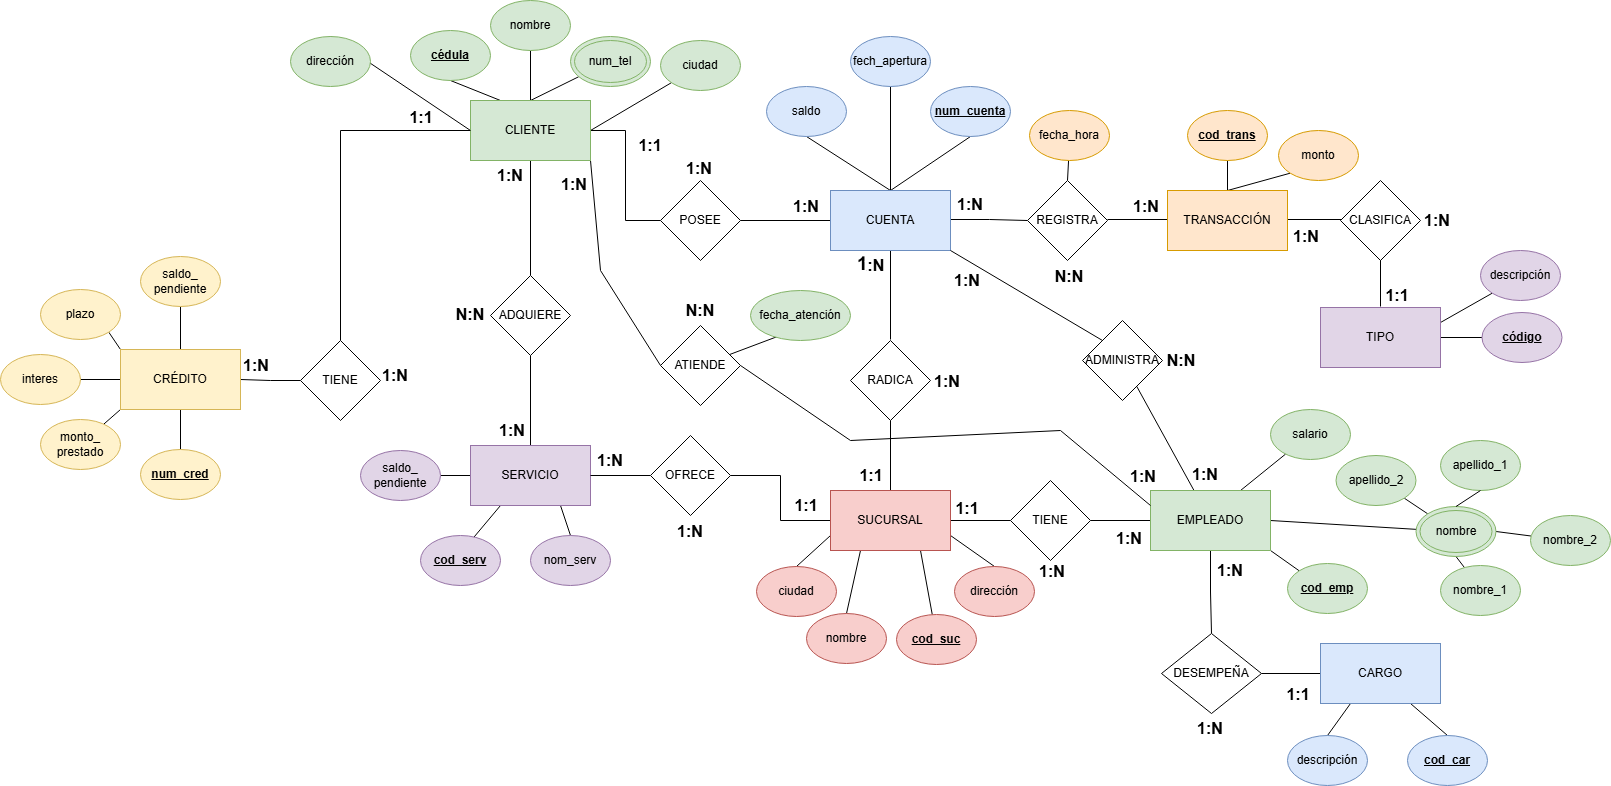
\includegraphics[width=\textwidth]{../diagramas/conceptual.png}
\caption{Diseño conceptual del sistema propuesto.}
\label{fig:dc}
\end{figure}

\section{Construcción del Diseño Lógico}

Una vez construido el modelo conceptual, se procede a su transformación en un modelo lógico relacional. De acuerdo con Elmasri y Navathe, este proceso consiste en convertir las entidades, atributos y relaciones identificados en el modelo Entidad--Relación en un conjunto de relaciones (tablas), definiendo además las claves primarias y foráneas necesarias para mantener la integridad de los datos \parencite{Elmasri2016}.

El resultado de este proceso se representa en la Figura \ref{fig:dl}.

\begin{figure}
\centering
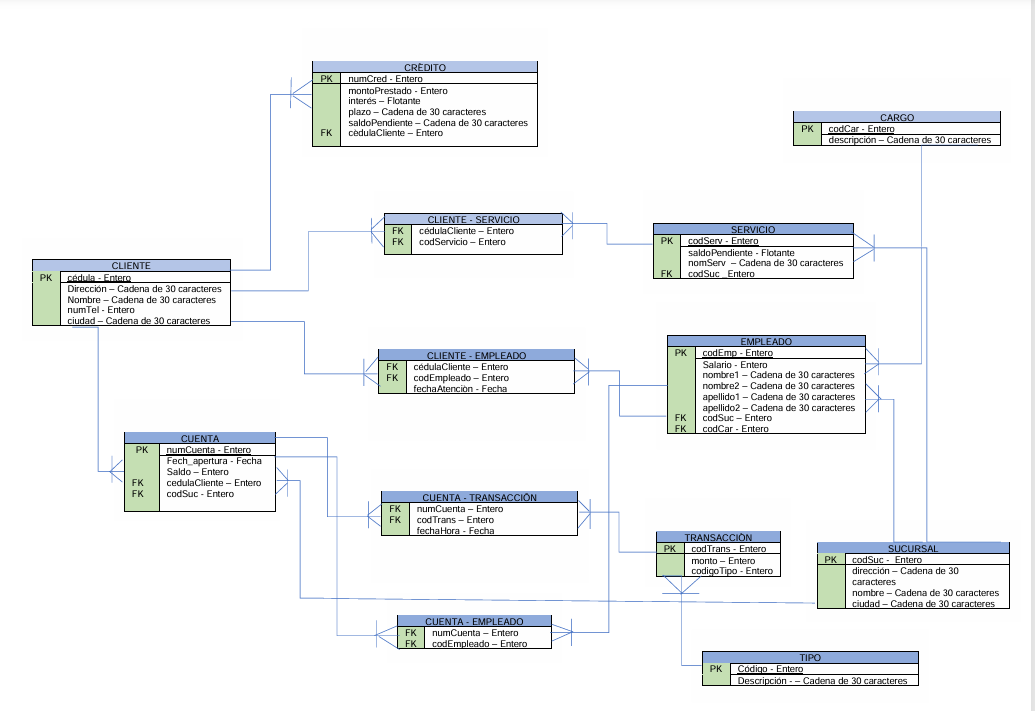
\includegraphics[width=\textwidth]{../diagramas/logico.png}
\caption{Diseño lógico del sistema propuesto.}
\label{fig:dl}
\end{figure}

Las imágenes en mejor resolución pueden consultarse en el siguiente enlace:

\begin{center}
   \href{https://github.com/jerofax/bd-operaciones-bancarias/tree/main/diagramas}{\textbf{Carpeta de diagramas en el repositorio}} 
\end{center}


\section{Consultas en Álgebra Relacional y Cálculo Relacional}

Las consultas constituyen uno de los principales mecanismos para el análisis de información en una base de datos. De acuerdo con Elmasri y Navathe, el Álgebra Relacional proporciona un conjunto de operadores que permiten manipular relaciones y obtener nueva información a partir de los datos existentes, mientras que el Cálculo Relacional ofrece un enfoque declarativo basado en predicados lógicos para expresar consultas \parencite{Elmasri2016}.

Con el propósito de validar la estructura propuesta para la base de datos de Bancolombia, se formularon las siguientes consultas utilizando operadores del Álgebra Relacional y expresiones de Cálculo Relacional. Estas consultas permiten recuperar información relevante relacionada con clientes, cuentas, transacciones, sucursales, empleados y servicios adicionales, incluyendo operaciones que involucran la combinación de múltiples relaciones del esquema diseñado.

\subsection{Consulta 1}
Mostrar los clientes de la ciudad de Medellín.

\subsubsection{Álgebra Relacional}

\[
\sigma_{ciudad='Medellín'}(CLIENTE)
\]

\subsubsection{Cálculo Relacional}

\[
\{t \mid CLIENTE(t) \land t.ciudad='Medellín'\}
\]

%%%%%%%%%%%%%%%%%%%%%%%%%%%%%%%%%%%%%%%%%%%%%%%%%%

\subsection{Consulta 2}
Mostrar únicamente el nombre y la ciudad de los clientes.

\subsubsection{Álgebra Relacional}

\[
\pi_{nombre,ciudad}(CLIENTE)
\]

\subsubsection{Cálculo Relacional}

\[
\{t.nombre,t.ciudad \mid CLIENTE(t)\}
\]

%%%%%%%%%%%%%%%%%%%%%%%%%%%%%%%%%%%%%%%%%%%%%%%%%%

\subsection{Consulta 3}
Mostrar los clientes que viven en Medellín o Bogotá.

\subsubsection{Álgebra Relacional}

\[
\pi_{cedula,nombre}
(\sigma_{ciudad='Medellín'}(CLIENTE))
\cup
\pi_{cedula,nombre}
(\sigma_{ciudad='Bogotá'}(CLIENTE))
\]

\subsubsection{Cálculo Relacional}

\[
\{t \mid CLIENTE(t)
\land
(t.ciudad='Medellín'
\lor
t.ciudad='Bogotá')
\}
\]

%%%%%%%%%%%%%%%%%%%%%%%%%%%%%%%%%%%%%%%%%%%%%%%%%%

\subsection{Consulta 4}
Mostrar los clientes que tienen cuenta pero no tienen crédito.

\subsubsection{Álgebra Relacional}

\[
\pi_{cedulaCliente}(CUENTA)
-
\pi_{cedulaCliente}(CREDITO)
\]

\subsubsection{Cálculo Relacional}

\[
\{t \mid CUENTA(t)
\land
\neg(CREDITO(t))
\}
\]

%%%%%%%%%%%%%%%%%%%%%%%%%%%%%%%%%%%%%%%%%%%%%%%%%%

\subsection{Consulta 5}
Mostrar los clientes que poseen cuenta y crédito.

\subsubsection{Álgebra Relacional}

\[
\pi_{cedulaCliente}(CUENTA)
\cap
\pi_{cedulaCliente}(CREDITO)
\]

\subsubsection{Cálculo Relacional}

\[
\{t \mid CUENTA(t)
\land
CREDITO(t)
\}
\]

%%%%%%%%%%%%%%%%%%%%%%%%%%%%%%%%%%%%%%%%%%%%%%%%%%

\subsection{Consulta 6}
Realizar el producto cartesiano entre CLIENTE y SUCURSAL.

\subsubsection{Álgebra Relacional}

\[
CLIENTE \times SUCURSAL
\]

\subsubsection{Cálculo Relacional}

\[
\{t \mid CLIENTE(c)
\land
SUCURSAL(s)\}
\]

%%%%%%%%%%%%%%%%%%%%%%%%%%%%%%%%%%%%%%%%%%%%%%%%%%

\subsection{Consulta 7}
Mostrar los clientes que poseen créditos registrados.

\subsubsection{Álgebra Relacional}

\[
CLIENTE \bowtie CREDITO
\]

\subsubsection{Cálculo Relacional}

\[
\{t \mid
CLIENTE(c)
\land
CREDITO(cr)
\land
c.cedula=cr.cedulaCliente
\}
\]

%%%%%%%%%%%%%%%%%%%%%%%%%%%%%%%%%%%%%%%%%%%%%%%%%%

\subsection{Consulta 8}
Mostrar los empleados y la sucursal a la que pertenecen.

\subsubsection{Álgebra Relacional}

\[
EMPLEADO \bowtie SUCURSAL
\]

\subsubsection{Cálculo Relacional}

\[
\{t \mid
EMPLEADO(e)
\land
SUCURSAL(s)
\land
e.codSuc=s.codSuc
\}
\]

%%%%%%%%%%%%%%%%%%%%%%%%%%%%%%%%%%%%%%%%%%%%%%%%%%

\subsection{Consulta 9}
Mostrar los empleados que trabajan en sucursales ubicadas en Medellín.

\subsubsection{Álgebra Relacional}

\[
EMPLEADO
\bowtie_{EMPLEADO.codSuc=SUCURSAL.codSuc}
\sigma_{ciudad='Medellín'}(SUCURSAL)
\]

\subsubsection{Cálculo Relacional}

\[
\{t \mid
EMPLEADO(e)
\land
SUCURSAL(s)
\land
e.codSuc=s.codSuc
\land
s.ciudad='Medellín'
\}
\]

%%%%%%%%%%%%%%%%%%%%%%%%%%%%%%%%%%%%%%%%%%%%%%%%%%


%%%%%%%%%%%%%%%%%%%%%%%%%%%%%%%%%%%%%%%%%%%%%%%%%%

\subsection{Consulta 10}
Mostrar los clientes que tienen tanto una cuenta como un crédito.

\subsubsection{Álgebra Relacional}

\[
\pi_{cedulaCliente}(CUENTA)
\cap
\pi_{cedulaCliente}(CREDITO)
\]

\subsubsection{Cálculo Relacional}

\[
\{t \mid
CUENTA(t)
\land
CREDITO(t)
\}
\]

%%%%%%%%%%%%%%%%%%%%%%%%%%%%%%%%%%%%%%%%%%%%%%%%%%

\subsection{Consulta 11}
Mostrar los clientes que tienen cuenta bancaria pero no tienen servicios registrados.

\subsubsection{Álgebra Relacional}

\[
\pi_{cedulaCliente}(CUENTA)
-
\pi_{cedulaCliente}(CLIENTE\_SERVICIO)
\]

\subsubsection{Cálculo Relacional}

\[
\{t \mid
CUENTA(t)
\land
\neg CLIENTE\_SERVICIO(t)
\}
\]

%%%%%%%%%%%%%%%%%%%%%%%%%%%%%%%%%%%%%%%%%%%%%%%%%%

\subsection{Consulta 12}
Renombrar la tabla CLIENTE como USUARIO.

\subsubsection{Álgebra Relacional}

\[
\rho_{USUARIO}(CLIENTE)
\]

\subsubsection{Cálculo Relacional}

\[
\{t \mid USUARIO(t)\}
\]


\section{Conclusiones}

El desarrollo del presente proyecto permitió aplicar los conceptos fundamentales del diseño de bases de datos relacionales a un caso de estudio basado en una entidad financiera de gran escala como Bancolombia. A partir del análisis de los requerimientos identificados, fue posible construir un modelo conceptual mediante el uso del Modelo Entidad-Relación y posteriormente transformarlo en un esquema relacional adecuado para la gestión de la información.

El diseño propuesto permite representar de manera estructurada los datos asociados a clientes, cuentas, transacciones, sucursales y empleados, definiendo las relaciones necesarias para garantizar la integridad y consistencia de la información. Asimismo, la identificación de claves primarias, claves foráneas y relaciones entre entidades contribuye a una organización eficiente de los datos dentro del sistema.

Finalmente, la formulación de consultas mediante Álgebra Relacional y Cálculo Relacional permitió evidenciar la utilidad del modelo diseñado para la recuperación de información relevante, demostrando la importancia de una adecuada etapa de modelado dentro del proceso de construcción de una base de datos.


\printbibliography

\end{document}

%% 
%% Copyright (C) 2019 by Daniel A. Weiss <daniel.weiss.led at gmail.com>
%% 
%% This work may be distributed and/or modified under the
%% conditions of the LaTeX Project Public License (LPPL), either
%% version 1.3c of this license or (at your option) any later
%% version.  The latest version of this license is in the file:
%% 
%% http://www.latex-project.org/lppl.txt
%% 
%% Users may freely modify these files without permission, as long as the
%% copyright line and this statement are maintained intact.
%% 
%% This work is not endorsed by, affiliated with, or probably even known
%% by, the American Psychological Association.
%% 
%% This work is "maintained" (as per LPPL maintenance status) by
%% Daniel A. Weiss.
%% 
%% This work consists of the file  apa7.dtx
%% and the derived files           apa7.ins,
%%                                 apa7.cls,
%%                                 apa7.pdf,
%%                                 README,
%%                                 APA7american.txt,
%%                                 APA7british.txt,
%%                                 APA7dutch.txt,
%%                                 APA7english.txt,
%%                                 APA7german.txt,
%%                                 APA7ngerman.txt,
%%                                 APA7greek.txt,
%%                                 APA7czech.txt,
%%                                 APA7turkish.txt,
%%                                 APA7endfloat.cfg,
%%                                 Figure1.pdf,
%%                                 shortsample.tex,
%%                                 longsample.tex, and
%%                                 bibliography.bib.
%% 
%%
%%
%% This is file `./samples/shortsample.tex',
%% generated with the docstrip utility.
%%
%% The original source files were:
%%
%% apa7.dtx  (with options: `shortsample')
%% ----------------------------------------------------------------------
%% 
%% apa7 - A LaTeX class for formatting documents in compliance with the
%% American Psychological Association's Publication Manual, 7th edition
%% 
%% Copyright (C) 2019 by Daniel A. Weiss <daniel.weiss.led at gmail.com>
%% 
%% This work may be distributed and/or modified under the
%% conditions of the LaTeX Project Public License (LPPL), either
%% version 1.3c of this license or (at your option) any later
%% version.  The latest version of this license is in the file:
%% 
%% http://www.latex-project.org/lppl.txt
%% 
%% Users may freely modify these files without permission, as long as the
%% copyright line and this statement are maintained intact.
%% 
%% This work is not endorsed by, affiliated with, or probably even known
%% by, the American Psychological Association.
%% 
%% ----------------------------------------------------------------------